% Source: Lecture9.pdf, pages 1-5 (page 6 is blank).
\lecture{9}

We discuss Potts models further here, including an interesting application of Potts
antiferromagnets.

\subsection{Chromatic polynomials and ground-state entropy}
\subsubsection*{Chromatic polynomials from deletion--contraction}

Recall from the previous lecture that, with $v = e^{K_P}-1$,
\begin{equation}
  Z(G,q,v=-1) = P(G,q),
\end{equation}
i.e.\ $Z$ of the zero-temperature Potts antiferromagnet (AFM) on a graph $G$ is precisely the
chromatic polynomial of $G$, enumerating the number of proper $q$-colorings of the vertices of
$G$ with $q$ colors.

The deletion--contraction relation (DCR) provides a way to calculate $P(G,q)$ for any $G$:
\begin{equation}
  P(G,q) = P(G-e,q) - P(G/e,q).
\end{equation}
This can be used iteratively, and at each step, the graphs on the RHS, $G-e$ and $G/e$, involve
one less edge. Hence eventually one is left with $E_n$, for which one has $P(E_n,q) = q^n$.

Example: we previously calculated $Z(C_n,q,v) = (q+v)^n + (q-1)v^n$, so, as a special case,
\begin{equation}
  P(C_n,q) = Z(C_n,q,v=-1) = (q-1)^n + (q-1)(-1)^n .
\end{equation}
Now let us see how this can be derived directly without going through the more complicated
$Z(C_n,q,v)$. Recall that $P(K_3,q) = q(q-1)(q-2)$. Use the DCR to calculate $P(C_4,q)$,
marking the edge to be deleted with a cross:
\begin{equation}
  P(C_4,q) = P(T_4,q) - P(K_3,q),\qquad K_3 = C_3 ,
\end{equation}
since deleting an edge of the square $C_4$ leaves a path (a tree $T_4$), and contracting it
leaves a triangle.

\paragraph{Lemma.} Let $T_n$ be a tree graph with $n$ vertices. Then
$P(T_n,q) = q(q-1)^{n-1}$.

E.g.\ take one example of $T_5$: a path $v_1v_2v_4v_5$ with a vertex $v_3$ attached to $v_2$.
We can pick one of the end vertices and assign any of the $q$ colors to it; let's take $v_1$.
Next, we go on to the adjacent vertex $v_2$; we can use any of the other $q-1$ colors for this
vertex. Next, we can independently assign any of the other $q-1$ colors different from
$q(v_2)$ to $q(v_3)$ and $q(v_4)$. Note that $q(v_1)$ may be equal to $q(v_3)$ or to $q(v_4)$,
since $v_1$ is not adjacent to $v_3$ or $v_4$, and also note that $q(v_3)$ may be equal to
$q(v_4)$, since $v_3$ and $v_4$ are not adjacent. Then one can choose $q(v_5)$ from $q-1$
colors, since the only constraint on this choice is that $q(v_5)\ne q(v_4)$. So
$P(T_5,q) = q(q-1)^4$. Generalizing this, $P(T_n,q) = q(q-1)^{n-1}$.

Now substitute:
\begin{align}
  P(C_4,q) &= P(T_4,q) - P(K_3,q) = q(q-1)^3 - q(q-1)(q-2)\nonumber\\
           &= q(q-1)\left[(q-1)^2-(q-2)\right]\nonumber\\
           &= q(q-1)\left[q^2-3q+3\right] = (q-1)^4 + (q-1)(-1)^4 ,
\end{align}
using $(q-1)^2-(q-2) = q^2-2q+1-q+2 = q^2-3q+3$.

Next proceed inductively:
\begin{equation}
  P(C_5,q) = P(T_5,q) - P(C_4,q);
\end{equation}
we have calculated both of these, so we get $P(C_5,q)$. Etc.:
\begin{equation}
  P(C_n,q) = P(T_n,q) - P(C_{n-1},q)
\end{equation}
$\Rightarrow$ the general result for $P(C_n,q)$ by iterative use of the DCR.

Recall
\begin{equation}
  Z(G,q,v) = \sum_{G'\subseteq G}q^{k(G')}v^{e(G')}
\end{equation}
$\Rightarrow$
\begin{align*}
  \max\deg_q(Z) &= k(E_n) = n(G); & \max\deg_v(Z) &= e(G);\\
  \min\deg_q(Z) &= k(G) = 1; & \min\deg_v(Z) &= e(E_n) = 0 .
\end{align*}
Since $P(G,q) = Z(G,q,v=-1)$, $\Rightarrow\max\deg_q(P) = n(G)$, since $k(E_n)$ does not
depend on $v$; and $\min\deg_q(P) = 1$.

\subsubsection*{Ground-state entropy of the Potts antiferromagnet}

Next, apply these methods to derive an important result in stat.\ mech.\ and thermodynamics.
Consider the $q$-state Potts AFM with $H = 0$ on a bipartite graph,
$G_{\text{bip.}} = G_1\oplus G_2$. We will derive a lower bound on
$Z(G_{\text{bip.}},q,v=-1) = P(G_{\text{bip.}},q)$, the $T = 0$ Potts AFM. A lower bound on
$P(G_{\text{bip.}},q)$ is obtained by assigning one color to all vertices $v_i\in G_1$. This can
be done in any of $q$ ways. Then, independently for each vertex $v_i\in G_2$, we can assign a
color from the remaining set of $q-1$ colors. There are $\frac n2$ vertices in $G_1$ and
$\frac n2$ vertices in $G_2$. So
\begin{equation}
  P(G_{\text{bip.}},q)\ge q(q-1)^{n/2},\qquad\text{where } n = n(G_{\text{bip.}}).
\end{equation}

\begin{diagram}
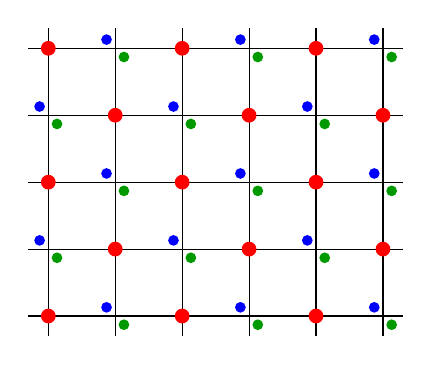
\begin{tikzpicture}[scale=0.85]
  \foreach \x in {0,...,5} \draw (\x,-0.3) -- (\x,4.3);
  \foreach \y in {0,...,4} \draw (-0.3,\y) -- (5.3,\y);
  \foreach \x in {0,...,5} \foreach \y in {0,...,4} {
    \pgfmathtruncatemacro{\prty}{mod(\x+\y,2)}
    \ifnum\prty=0
      \fill[red] (\x,\y) circle (0.11);
    \else
      \fill[blue] (\x-0.13,\y+0.13) circle (0.08);
      \fill[green!60!black] (\x+0.13,\y-0.13) circle (0.08);
    \fi}
\end{tikzpicture}
\diagramcaption{A section of the square lattice with $q = 3$ (red, green, blue). Red is
assigned to all $v_i\in G_1$; then for each $v_j\in G_2$ we can independently choose the color to
be either of the $q-1 = 2$ remaining colors, green or blue. So here
$P(G,3)\ge 3\cdot 2^{n/2} = 3\cdot 2^{15}$, since $n = 30$.}
\end{diagram}

In the general-$q$ case, all of these color assignments (spin states) minimize the energy of the
$q$-state Potts AFM, i.e.\ they are all degenerate ground states of the model.

Given that $Z(G_{\text{bip.}},q,v=-1)\ge q(q-1)^{n/2}$, this means that the $q$-state Potts AFM
(with $H = 0$, zero external magnetic field) has at least this much ground-state degeneracy for
$q\ge 3$. The ground-state degeneracy per site in the thermodynamic limit on a graph $G$ (say
$G$ = lattice $\Lambda$) is, for the Potts AFM,
\begin{equation}
  W(\Lambda,q) = \lim_{n\to\infty}\left[Z(\Lambda,q,v=-1)\right]^{1/n}
              = \lim_{n\to\infty}\left[P(\Lambda,q)\right]^{1/n},
\end{equation}
and the corresponding ground-state entropy per site $\bar S_0$ is
\begin{equation}
  \bar S_0 = \kB\ln W .
\end{equation}
So for the $q$-state Potts AFM on $\Lambda_{\text{bip.}}$,
\begin{equation}
  W(\Lambda_{\text{bip.}},q)_{\text{Potts AFM}}\ge\lim_{n\to\infty}\left[q(q-1)^{n/2}\right]^{1/n}\ge(q-1)^{1/2}
\end{equation}
(using $\lim_{n\to\infty}q^{1/n} = 1$ for $q\ne 0$), and hence
\begin{equation}
  \bar S_0(\Lambda_{\text{bip.}},q)_{\text{Potts AFM}}\ge\frac{\kB}{2}\ln(q-1)>0\quad\text{for } q\ge 3,
\end{equation}
i.e.\ the entropy per site of the $q$-state Potts AFM with $q\ge 3$ is nonzero. This is a
counterexample to the so-called Third ``Law'' of Thermodynamics, which states that
$\bar S_0 = 0$. The fact that this ``law'' has exceptions is well known in stat.\ mech.\ but is
not usually mentioned in elementary physics books.

\subsubsection*{Residual entropy of ice}

Ice is a physical example of nonzero ground state entropy (called $T = 0$ residual entropy in
chemistry). Recall that ice is a hydrogen-bonded molecular crystal and (at $p\sim 1$~atm,
$T\lesssim 0^\circ$C) has a wurtzite crystal structure with tetragonal bonding. On each hydrogen
bond one has an electric dipole; indicate the direction of the electric dipole with an arrow.

Because the bonding is tetragonal, we can represent each oxygen atom as a vertex with degree 4.
Each oxygen atom has 2 hydrogens bonded to it, hence 2 electric dipoles pointing in and 2
electric dipoles pointing out. We represent these as arrows
($\leftarrow,\uparrow,\rightarrow,\downarrow$). The bond angles are not $90^\circ$ and the
crystal structure is not 2-dimensional, but our diagram for a given oxygen atom (vertex with 4
bonds) correctly represents the physics. The Slater Rule, also called the requirement of local
electric neutrality, stipulates that 2 of the 4 arrows must point outward and the other 2
inward. The total number of arrow configurations at each vertex is $2^4 = 16$, but only
$\binom42 = 6$ of these satisfy the constraint of local electric neutrality, where
$\binom ab = \frac{a!}{b!(a-b)!}$.

\begin{diagram}
\begin{tikzpicture}[scale=0.55,>=Stealth]
  % each entry: left, right, down, up arrows; 1 = pointing toward the center
  \foreach \n/\l/\r/\d/\u in {0/1/1/0/0, 1/0/0/1/1, 2/1/0/1/0, 3/1/0/0/1, 4/0/1/1/0, 5/0/1/0/1} {
    \begin{scope}[xshift=2.6*\n cm]
      \draw (-1,0) -- (1,0); \draw (0,-1) -- (0,1);
      \ifnum\l=1 \draw[->,blue,thick] (-1,0) -- (-0.35,0); \else \draw[->,blue,thick] (-0.35,0) -- (-1,0); \fi
      \ifnum\r=1 \draw[->,blue,thick] (1,0) -- (0.35,0); \else \draw[->,blue,thick] (0.35,0) -- (1,0); \fi
      \ifnum\d=1 \draw[->,blue,thick] (0,-1) -- (0,-0.35); \else \draw[->,blue,thick] (0,-0.35) -- (0,-1); \fi
      \ifnum\u=1 \draw[->,blue,thick] (0,1) -- (0,0.35); \else \draw[->,blue,thick] (0,0.35) -- (0,1); \fi
    \end{scope}}
\end{tikzpicture}
\diagramcaption{The $\binom42 = 6$ arrow configurations at a vertex allowed by local electric
neutrality (two arrows in, two out). The other 10 arrow configurations, e.g.\ four in or three
in and one out, are forbidden.}
\end{diagram}

The residual entropy of H$_2$O ice is measured to be
$S_0 = 0.82\ \frac{\text{cal}}{\text{mole}\cdot\text{K}}$, i.e.\ (using
$R = N_{\text{Avog.}}\kB = 1.99\ \frac{\text{cal}}{\text{K}\cdot\text{mole}}$) $S_0 = 0.41R$, so
the residual entropy per molecule is $S_0 = 0.41\kB$, so, from $S_0 = \kB\ln W$, i.e.\
$W = e^{S_0/\kB} = e^{0.41} = 1.5$.

Linus Pauling (who was awarded two Nobel Prizes, in Chemistry and Peace) developed a simple
model that yields a very good approximation to this measured value of $\bar S_0$: assume that we
can approximate the total ground state degeneracy (number of g.s.\ configurations of the arrows
on the bonds) as the total number, $2^{e(\Lambda)}$, times the factor arising from the
constraint of local electric neutrality at each vertex of the crystal lattice (i.e.\ each oxygen
atom), namely $\frac{6}{2^4} = \frac38$. Then
\begin{equation}
  Z\simeq 2^{e(\Lambda)}\left(\frac38\right)^{n(\Lambda)}.
\end{equation}
Now $e(\Lambda) = \frac{\Delta}{2}n(\Lambda) = 2n(\Lambda)$ since $\Delta = 4$, so
\begin{equation}
  Z\simeq\left(4\cdot\frac38\right)^{n(\Lambda)} = \left(\frac32\right)^{n(\Lambda)},
  \qquad\text{so}\quad W = \lim_{n(\Lambda)\to\infty}Z^{1/n(\Lambda)} = \frac32 = 1.5 .
\end{equation}
This agrees very well with the measured value of the residual entropy of ice.

References (measurements):
\begin{itemize}
  \item W.F.~Giauque and M.F.~Ashley, Phys.\ Rev.\ \textbf{43}, 81 (1933);
  \item W.F.~Giauque and E.L.~Stout, J.\ Am.\ Chem.\ Soc.\ \textbf{58}, 1144 (1936);
  \item L.~Pauling, \emph{The Nature of the Chemical Bond} (book), p.~467 (1960).
\end{itemize}
Later there have been studies of ``vertex models'' in stat.\ mech.\ as models of ferroelectric
materials, which exhibit a net electric polarization at sufficiently low temperature (e.g.\
KH$_2$PO$_4$, potassium dihydrogen phosphate).

Note that a nonzero ground state entropy results if the actual g.s.\ degeneracy grows like $c^n$
for $c>1$, i.e.\ \#~configurations $\sim c^n$, so $W = c$, $S_0 = \kB\ln W = \kB\ln c$. We have
given two different examples of this phenomenon:
\begin{enumerate}
  \item the $q$-state Potts AF on a bipartite lattice (sq, hc, sc, etc.) for $q\ge 3$, where we
    derived a lower bound on $S_0$ (further calculations give actual estimates of $S_0$ as a
    function of $q$ and $\Lambda_{\text{bip.}}$);
  \item ice and the Pauling model for $S_0$.
\end{enumerate}

\subsubsection*{Frustration}

An important property of both of these examples is that they do \emph{not} involve
frustration. Recall that frustration occurs if the interactions cannot minimize the internal
energy. E.g.:
\begin{enumerate}
  \item An antiferromagnetic spin model in a (uniform) external magnetic field, since the
    spin--spin interaction prefers staggered magnetic ordering, while the external magnetic field
    favors (uniform) magnetic ordering.
  \item An antiferromagnetic spin model on certain non-bipartite lattices, such as the
    triangular lattice. One can see this by considering spin states on a single triangle of the
    lattice; say the spin $\sigma_1$ at vertex 1 is $+$. Then to minimize the interaction energy
    on bonds $e_{12}$ and $e_{13}$ the spins at vertices 2 and 3 should be $-$. But that
    conflicts with the minimization of the spin--spin interaction energy on bond $e_{23}$; with
    this set of spin states,
    \begin{equation}
      \Ham = -J\sum_{e_{ij}}\sigma_i\sigma_j = +|J|\sum_{e_{ij}}\sigma_i\sigma_j
           = |J|(\sigma_1\sigma_2+\sigma_2\sigma_3+\sigma_3\sigma_1) = |J|(-1+1-1) = -|J| .
    \end{equation}
\end{enumerate}
In contrast the ferromagnet can achieve a lower energy with all of the spin--spin interactions
taking their preferred values: with all spins $+$ or all spins $-$,
$\Ham = -J\sum_{e_{ij}}\sigma_i\sigma_j = -3J$.

\begin{diagram}
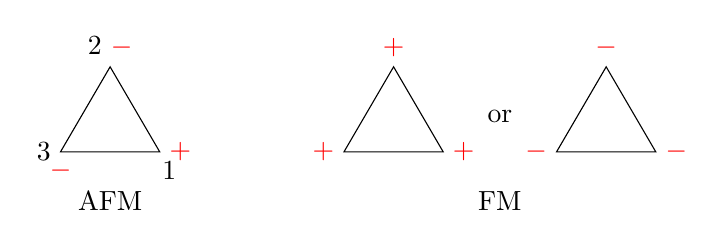
\begin{tikzpicture}[scale=0.9]
  \draw (0,0) -- (1.4,0) -- (0.7,1.2) -- cycle;
  \node[red,right] at (1.4,0) {$+$}; \node[left] at (0,0) {$3$}; \node[red,below] at (0,0) {$-$};
  \node[above] at (0.7,1.2) {$2\ {\color{red}-}$}; \node[below right] at (1.3,0) {$1$};
  \node at (0.7,-0.7) {AFM};
  \begin{scope}[xshift=4cm]
    \draw (0,0) -- (1.4,0) -- (0.7,1.2) -- cycle;
    \node[red,right] at (1.4,0) {$+$}; \node[red,left] at (0,0) {$+$}; \node[red,above] at (0.7,1.2) {$+$};
    \node at (2.2,0.5) {or};
    \begin{scope}[xshift=3cm]
      \draw (0,0) -- (1.4,0) -- (0.7,1.2) -- cycle;
      \node[red,right] at (1.4,0) {$-$}; \node[red,left] at (0,0) {$-$}; \node[red,above] at (0.7,1.2) {$-$};
    \end{scope}
    \node at (2.2,-0.7) {FM};
  \end{scope}
\end{tikzpicture}
\diagramcaption{A frustrated triangle for the Ising AFM, and the two FM ground states.}
\end{diagram}

As we will discuss later, this frustration in the Ising AFM on the triangular lattice drives
$T_c\to 0$.

Another example of a frustrated spin model is a ``spin glass'', where, e.g., the couplings
$J_{ij}$ have different signs on different bonds $e_{ij}$, with some being positive, favoring FM
ordering, and others being negative, favoring AFM ordering. Example: the Ising spin glass,
\begin{equation}
  \Ham = -\sum_{\{e_{ij}\}}\sigma_iJ_{ij}\sigma_j ,
\end{equation}
with the $J_{ij}$ random, distributed with equal probability $>0$ or $<0$: with probability
$\frac12$ for either sign, $J_{ij} = J$ or $-J$; or with a distribution $P(J_{ij})$ peaked
around $\pm J$, or a single broad distribution centered on zero, or a broad distribution with
peaks near $\pm J$.

\begin{diagram}
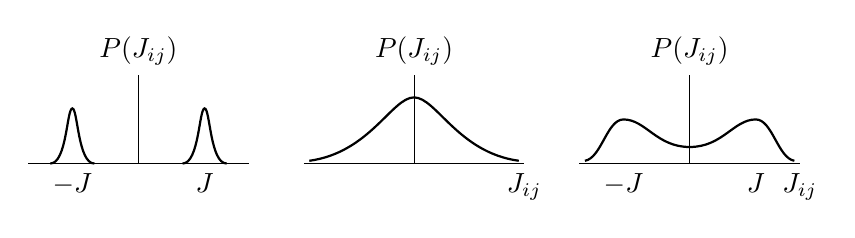
\begin{tikzpicture}[scale=0.7]
  \draw (-2,0) -- (2,0); \draw (0,0) -- (0,1.6) node[above] {$P(J_{ij})$};
  \draw[thick] (-1.6,0) .. controls (-1.3,0) and (-1.3,1) .. (-1.2,1) .. controls (-1.1,1) and (-1.1,0) .. (-0.8,0);
  \draw[thick] (0.8,0) .. controls (1.1,0) and (1.1,1) .. (1.2,1) .. controls (1.3,1) and (1.3,0) .. (1.6,0);
  \node[below] at (-1.2,0) {$-J$}; \node[below] at (1.2,0) {$J$};
  \begin{scope}[xshift=5cm]
    \draw (-2,0) -- (2,0) node[below] {$J_{ij}$}; \draw (0,0) -- (0,1.6) node[above] {$P(J_{ij})$};
    \draw[thick] (-1.9,0.05) .. controls (-0.8,0.2) and (-0.4,1.2) .. (0,1.2) .. controls (0.4,1.2) and (0.8,0.2) .. (1.9,0.05);
  \end{scope}
  \begin{scope}[xshift=10cm]
    \draw (-2,0) -- (2,0) node[below] {$J_{ij}$}; \draw (0,0) -- (0,1.6) node[above] {$P(J_{ij})$};
    \draw[thick] (-1.9,0.05) .. controls (-1.6,0.1) and (-1.5,0.8) .. (-1.2,0.8) .. controls (-0.8,0.8) and (-0.6,0.3) .. (0,0.3)
       .. controls (0.6,0.3) and (0.8,0.8) .. (1.2,0.8) .. controls (1.5,0.8) and (1.6,0.1) .. (1.9,0.05);
    \node[below] at (-1.2,0) {$-J$}; \node[below] at (1.2,0) {$J$};
  \end{scope}
\end{tikzpicture}
\diagramcaption{Possible distributions of the random couplings $J_{ij}$ in an Ising spin glass.}
\end{diagram}
